\chapter{\uppercase{Construção do Projeto}}
\label{Construção do Projeto}

\section{Técnologias Utilizadas}

 Inicialmente no projeto, as interações foram desenvolvidas dentro da plataforma Landbot, porém, devido a falta de atenção do grupo em não fazer uma pesquisa sobre a plataforma em questão, após o início do projeto, veio a conhecimento de que a Landbot não possuía um plano gratuito, apenas um período de teste. Outra plataforma considerada foi a IBM, porém esta não disponibiliza um plano gratuito sem o cadastro de um cartão de crédito. \cite{ibm}
 
 Devido a este contratempo, foi necessário fazer uma nova pesquisa de plataformas. Na escolha da plataforma Code7 Boteria, foram levadas em consideração: a disponibilidade de um plano gratuito amplo, possuir opções de coleta de informações disponibilizadas em relatórios e a opção para que o usuário possa dar dicas de falhas e sugestões para melhorias no BOT.

 Após mais pesquisas foi decidido pelo grupo uma outra plataforma, a plataforma escolhida foi a WhatsAuto  \cite{whats}, uma plataforma em formato de aplicativo que se configura para se ter respostas automáticas de uma ampla grade de aplicativos, como mostra na figura abaixo:

\begin{figure}[!htb]
\centering
\captionsetup[subfigure]{labelformat=empty}
\caption{``Aplicativos Suportados''}
\begin{subfigure}{.5\textwidth}
\centering
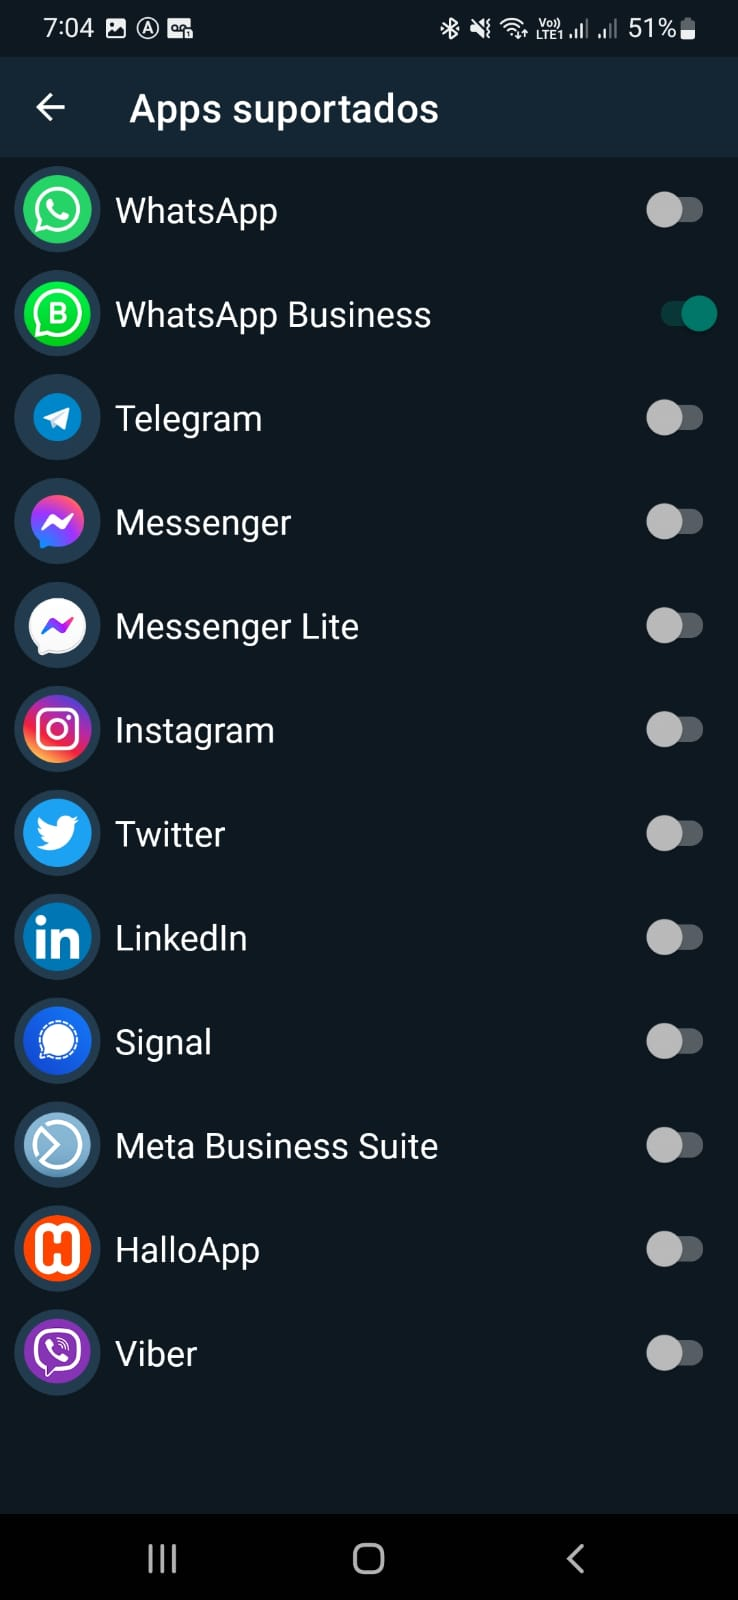
\includegraphics[width=6cm,height=9cm]{Partes/Imagens/Apps Suportados.jpeg}
\caption{Fonte: Criada pelo autor(2022).}
\end{subfigure}%
\end{figure}

Um ponto positivo para a nova plataforma é a facilidade para analisar as estatísticas de respostas, ou seja, o que os usuários mais estão acessando no BOT, dando uma ampla ideia do que melhorar futuramente ou dar mais informações:

\begin{figure}[!htb]
\centering
\captionsetup[subfigure]{labelformat=empty}
\caption{``Estatisticas de respostas''}
\begin{subfigure}{.5\textwidth}
\centering
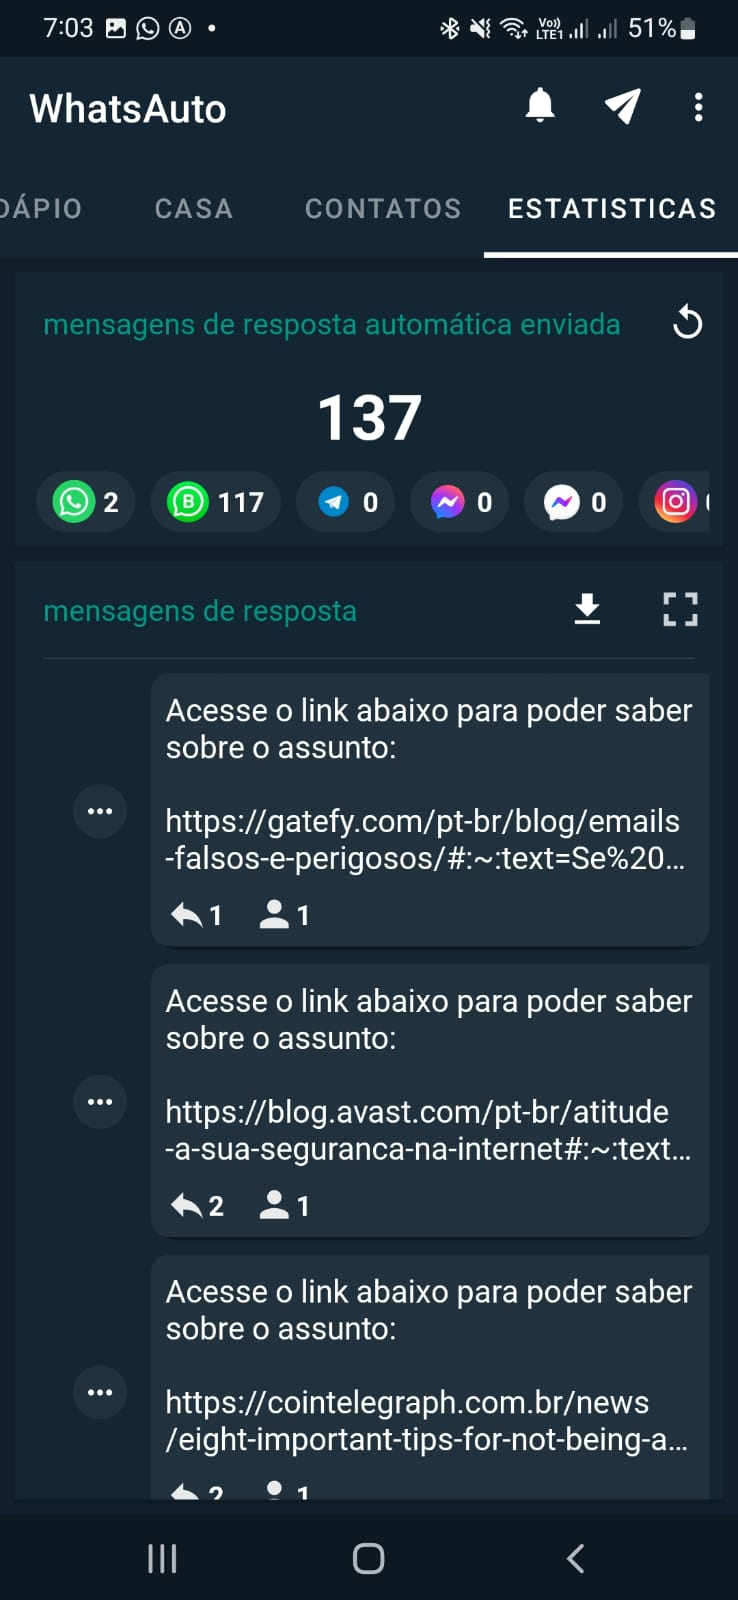
\includegraphics[width=6cm,height=9cm]{Partes/Imagens/Estatisticas.jpeg}
\caption{Fonte: Criada pelo autor(2022).}
\end{subfigure}%
\end{figure}

        \newpage
% Tecnologias utilizadas - Colocar as tecnologias utilizadas e os motivos das escolhas (se tiver custo coloque, se tiver limitação por ser trial, coloque).

% Desenhe um mapa de perguntas e respostas que o bot será capaz de responder.

\section{Protótipo}

A ideia para o nome do BOT veio das iniciais dos integrantes do grupo desenvolvedor, sendo eles: Guilherme, Isabelle, Vitor Hugo de Morais e Vitor Hugo Resende. Assim, foi criado o nome GUIV SECURITY BOT.

\begin{figure}[!htb]
\centering
\captionsetup[subfigure]{labelformat=empty}
\caption{``GUIV''}
\begin{subfigure}{.5\textwidth}
\centering

\includegraphics[width=8cm,height=6cm]{Partes/Imagens/Guiv S.jpeg}
\caption{Fonte: Criada pelo autor(2022).}
\end{subfigure}%
\end{figure}

\begin{itemize}

		\item \textbf{Passo a passo}: 

        O BOT utilizado é um aplicativo de respostas automáticas, que tem vários tipos de modos de respostas como mostra abaixo: \newpage	

\begin{figure}[!htb]
\centering
\captionsetup[subfigure]{labelformat=empty}
\caption{``Opções''}
\begin{subfigure}{.5\textwidth}
\centering
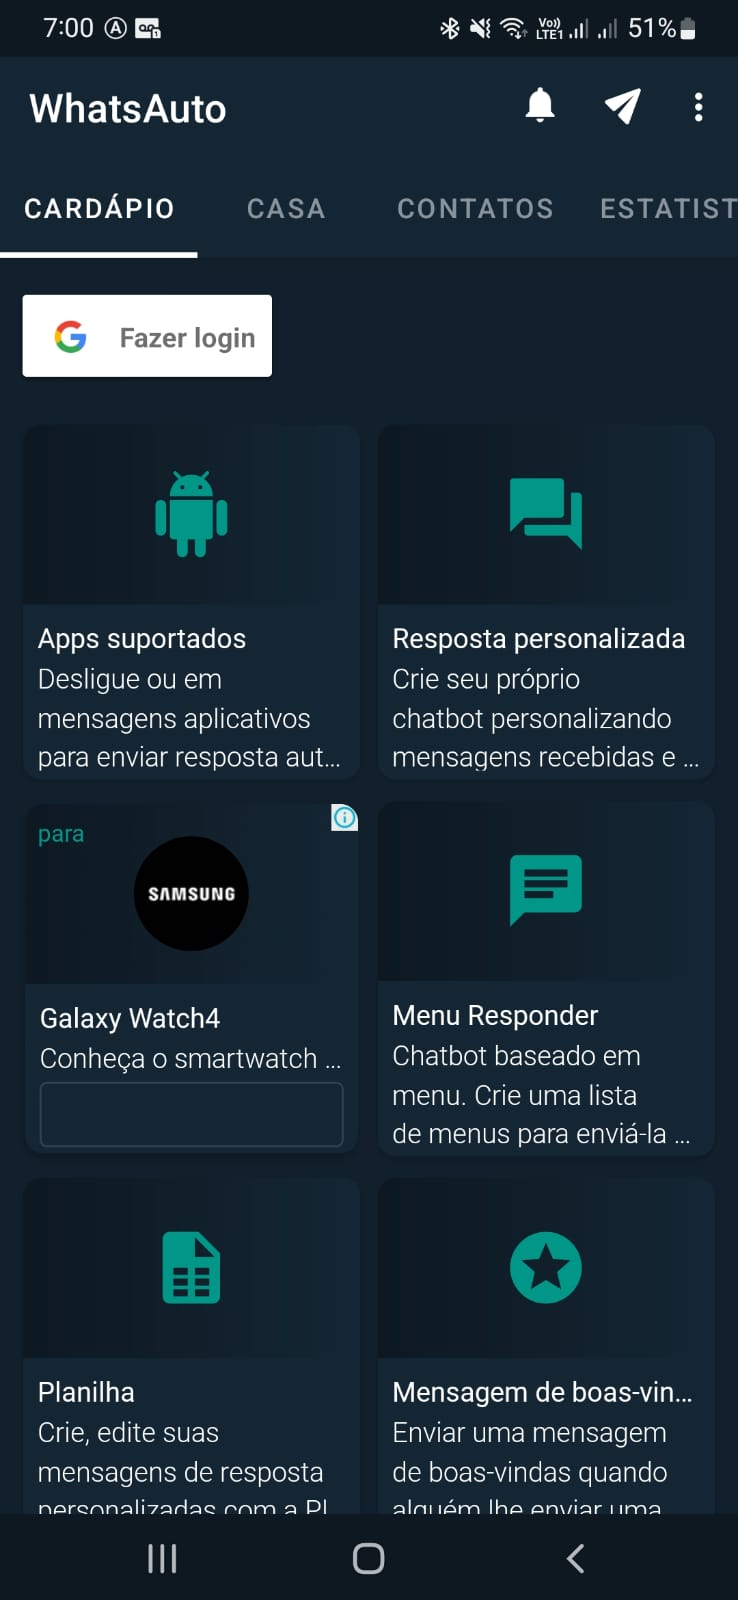
\includegraphics[width=6cm,height=8cm]{Partes/Imagens/Opções.jpeg}
\caption{Fonte: Whatsauto (2022).}
\end{subfigure}%
\end{figure}

        O modo que foi escolhido para fazer o BOT foi o de "Menu Responder", que é um tipo que o BOT te dá opções de respostas, mas além dele, tem opções de respostas que se derivam de mensagens específicas e outras. \\

        Para realizar a criação das opções que o BOT irá te dar para que se possa escolher e ter suas respostas, basta selecionar a opção "Menu Responder", que ele te direcionar a essa tela:  \newpage

\begin{figure}[!htb]
\centering
\captionsetup[subfigure]{labelformat=empty}
\caption{``Menu 1''}
\begin{subfigure}{.5\textwidth}
\centering
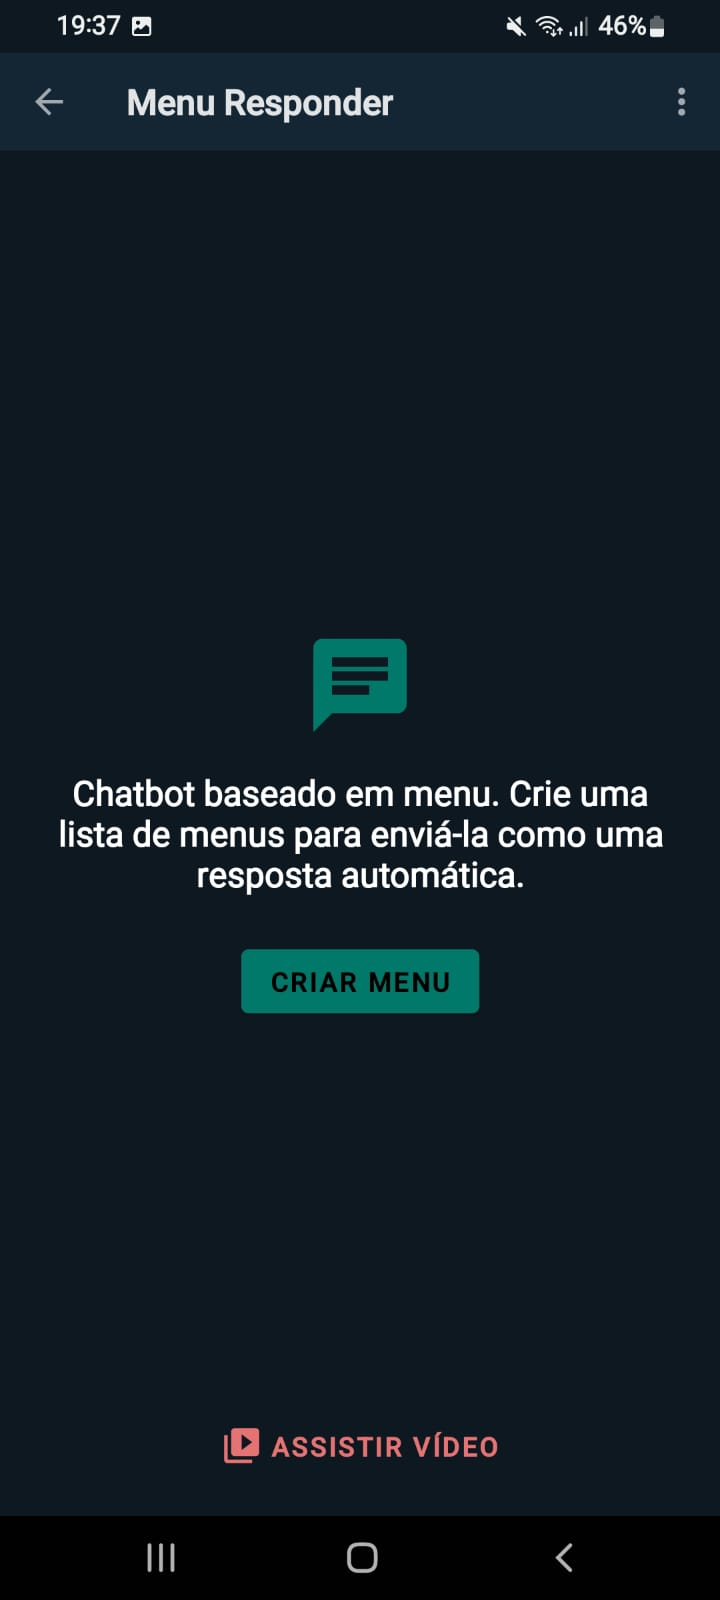
\includegraphics[width=6cm,height=8cm]{Partes/Imagens/Menu 1.jpeg}
\caption{Fonte: Whatsauto (2022).}
\end{subfigure}%
\end{figure}

        Ao abrir essa tela basta clicar em "Criar Menu" que ele te direcionará para a tela de criação:

\begin{figure}[!htb]
\centering
\captionsetup[subfigure]{labelformat=empty}
\caption{``Menu 2''}
\begin{subfigure}{.5\textwidth}
\centering
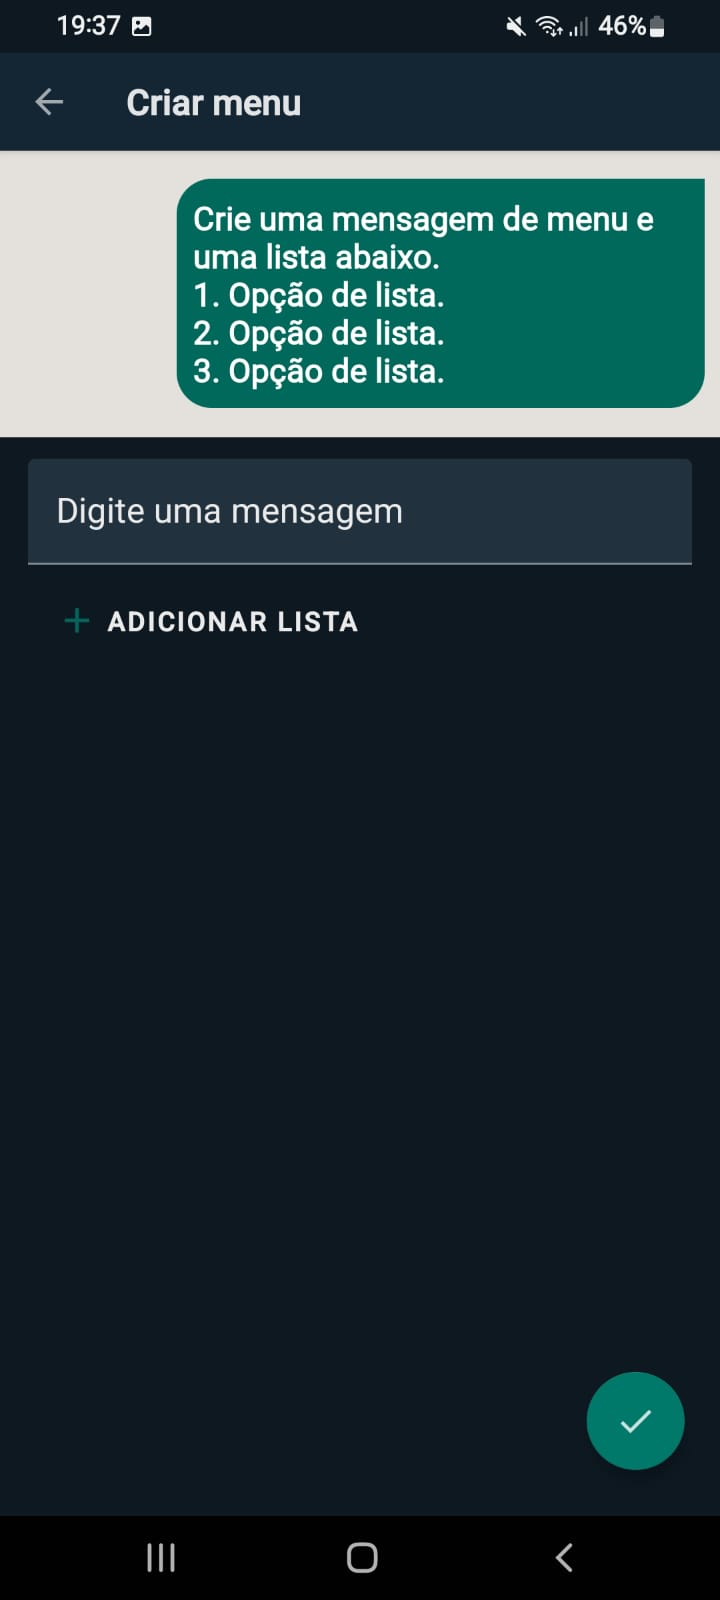
\includegraphics[width=6cm,height=8cm]{Partes/Imagens/Menu 2.jpeg}
\caption{Fonte: Whatsauto (2022).}
\end{subfigure}%
\end{figure}

        Nessa tela você irá colocar um texto inicial e as opções que terá no menu, colocando as informações e clicando na certo verde no canto inferior direito, você irá para a tela de menu criado: \newpage

\begin{figure}[!htb]
\centering
\captionsetup[subfigure]{labelformat=empty}
\caption{``Menu 3''}
\begin{subfigure}{.5\textwidth}
\centering
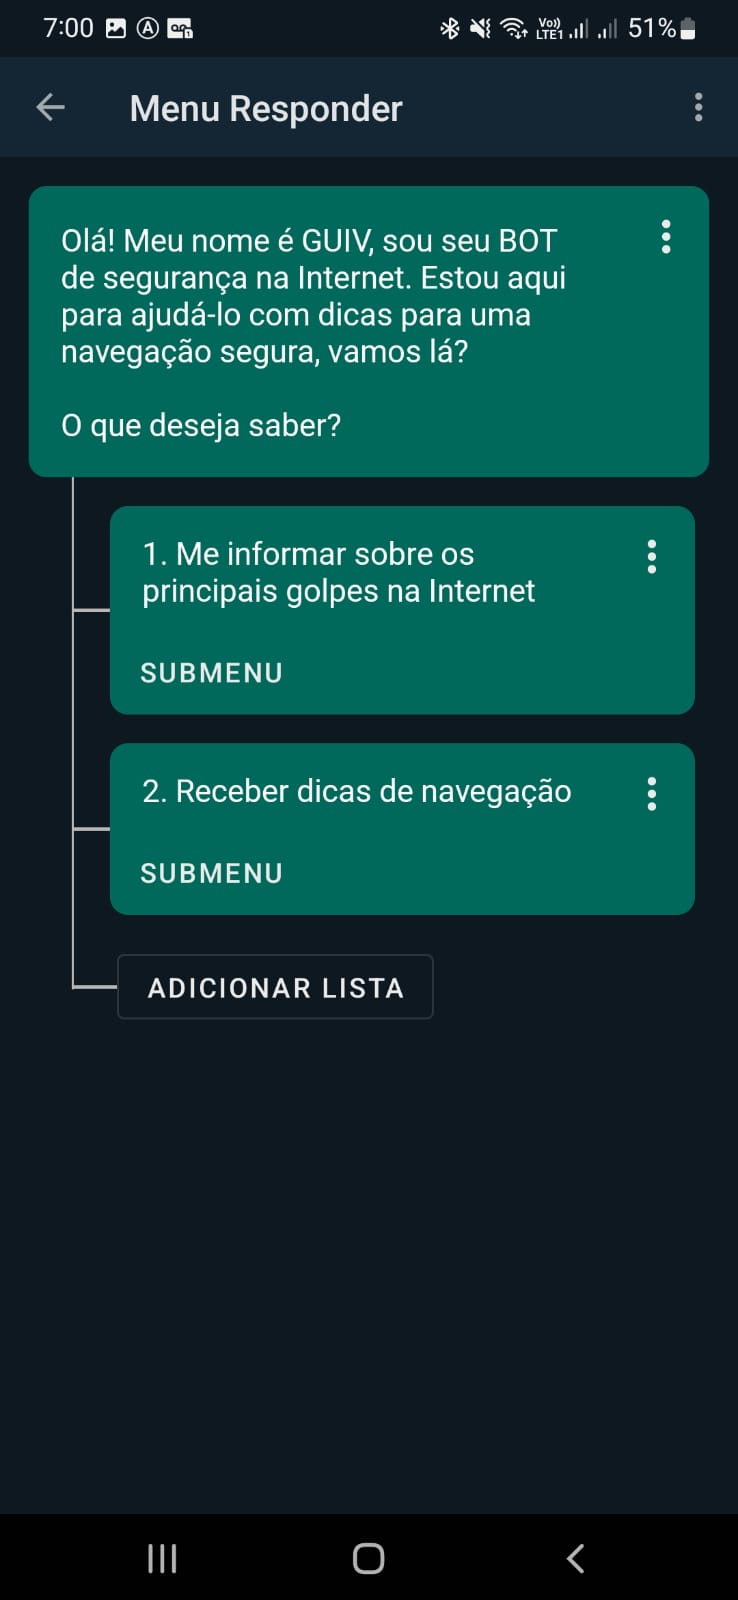
\includegraphics[width=6cm,height=8cm]{Partes/Imagens/Menu 3.jpeg}
\caption{Fonte: Whatsauto (2022).}
\end{subfigure}%
\end{figure}

        Mesmo depois de criado, se consegue editar e excluir as opções, basta clicar nos 3 pontinhos que ficam na direita de cada campo. \\

        Para que se crie as opções dentro de cada submenu, basta clicar em "SUBMENU" que fica em cada lista e ele te direcionará para a tela de criação dos submenus, que é igual a tela de criação do menu:

\begin{figure}[!htb]
\centering
\captionsetup[subfigure]{labelformat=empty}
\caption{``Submenu 1''}
\begin{subfigure}{.5\textwidth}
\centering
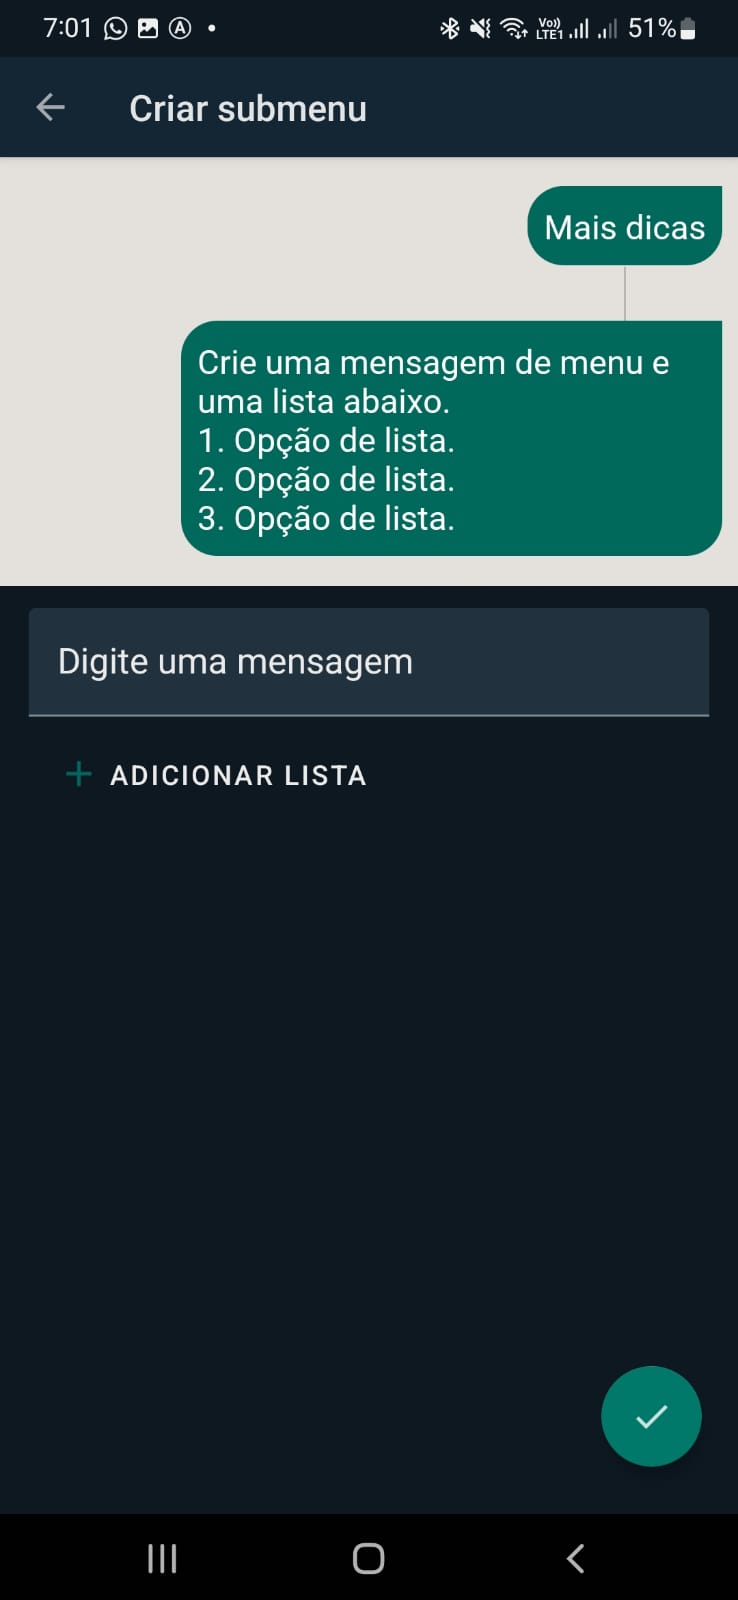
\includegraphics[width=6cm,height=8cm]{Partes/Imagens/Submenu 1.jpeg}
\caption{Fonte: Whatsauto (2022).}
\end{subfigure}%
\end{figure}


\begin{figure}[!htb]
\centering
\captionsetup[subfigure]{labelformat=empty}
\caption{``Submenu 2''}
\begin{subfigure}{.5\textwidth}
\centering
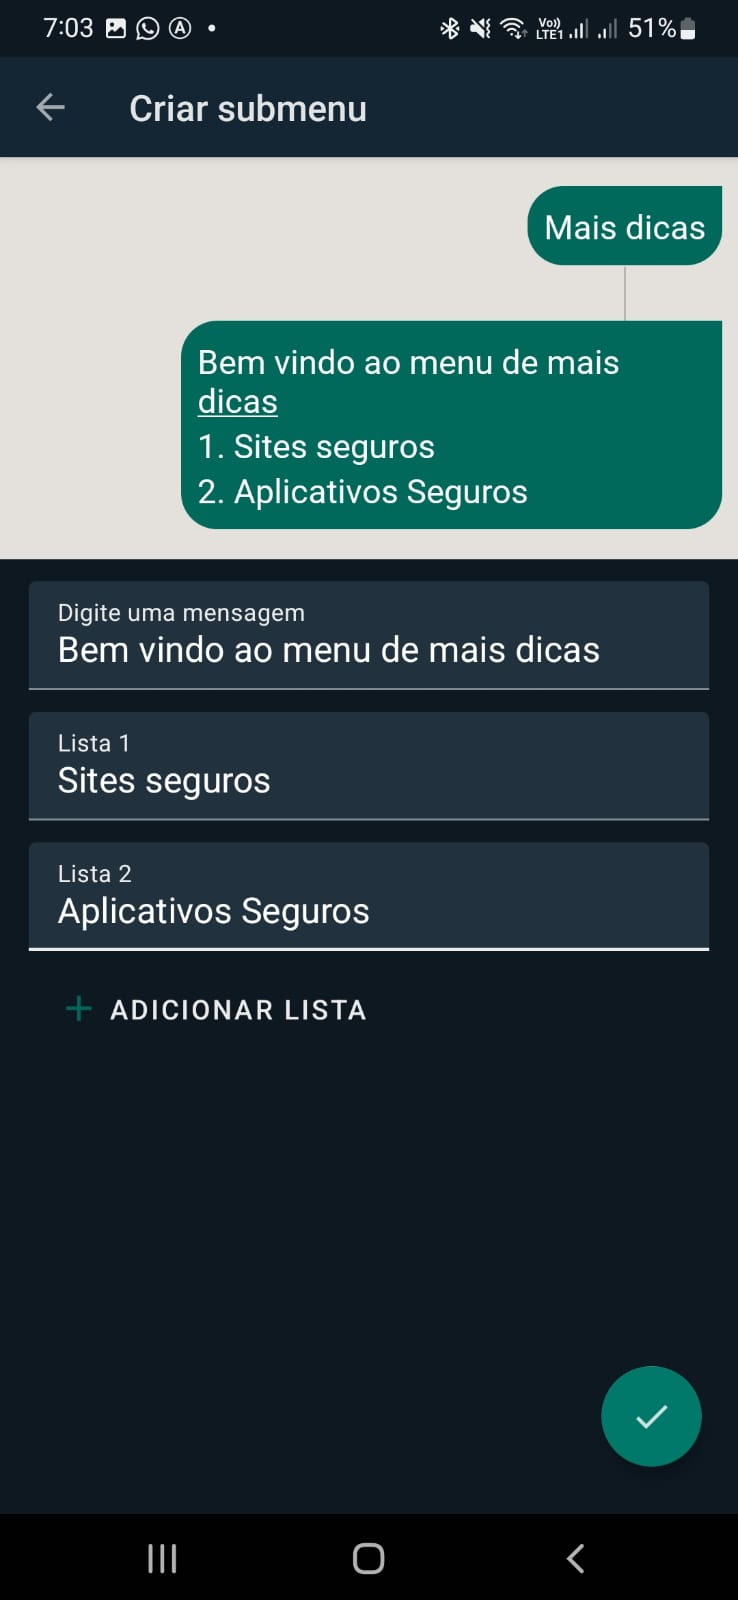
\includegraphics[width=6cm,height=8cm]{Partes/Imagens/Submenu 2.jpeg}
\caption{Fonte: Whatsauto (2022).}
\end{subfigure}%
\end{figure}

\begin{figure}[!htb]
\centering
\captionsetup[subfigure]{labelformat=empty}
\caption{``Submenu 3''}
\begin{subfigure}{.5\textwidth}
\centering
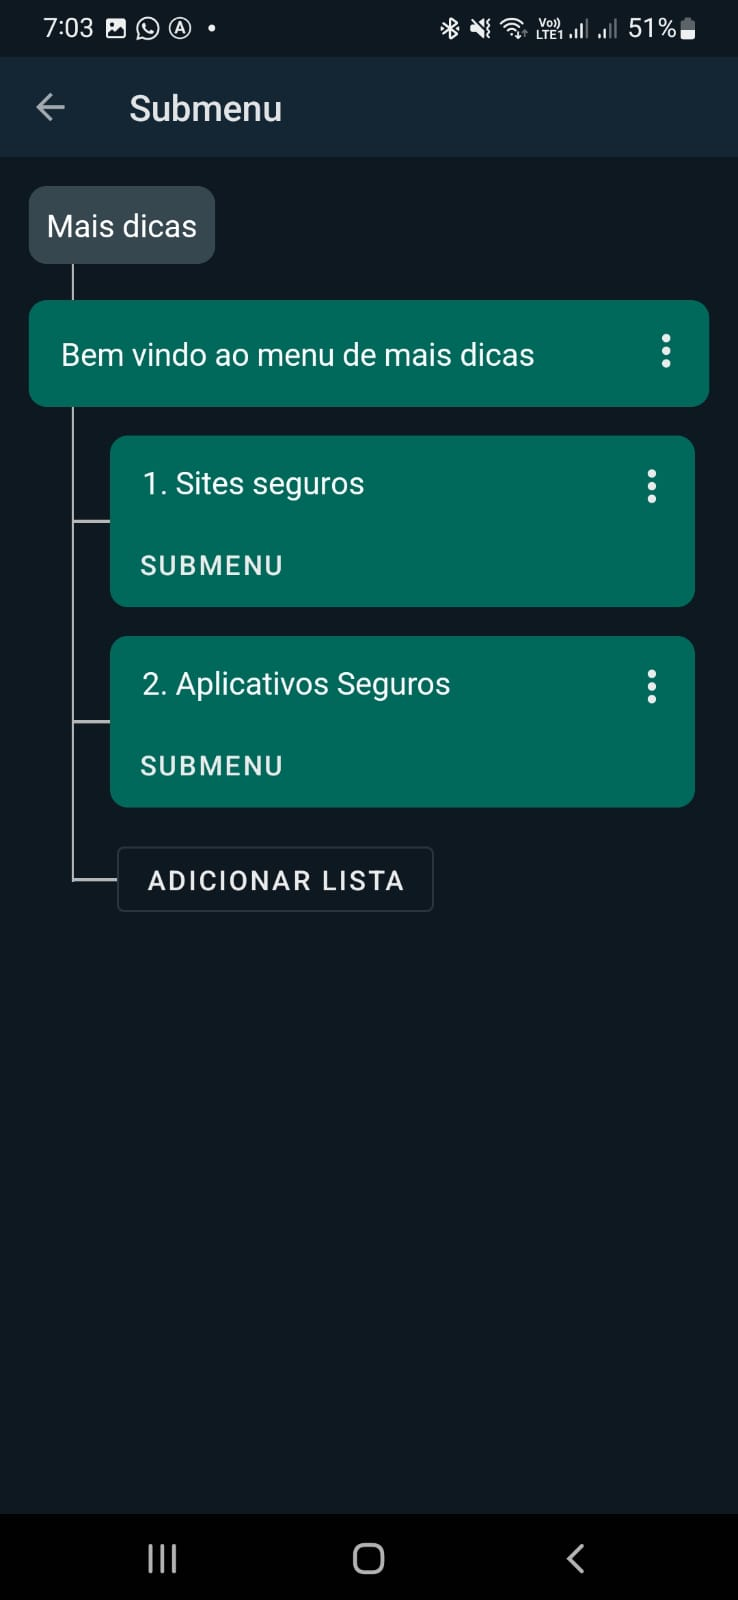
\includegraphics[width=6cm,height=8cm]{Partes/Imagens/Submenu 3.jpeg}
\caption{Fonte: Whatsauto (2022).}
\end{subfigure}%
\end{figure}

        \newpage
        
        Preenchendo os campos de texto e das listas seu submenu estará criado, podendo criar mais submenus dentro dele.
        
        Para colocar o BOT no ar, basta voltar para a tela de seleção do tipo de configuração e ir na categoria CASA na parte superior do aplicativo, dentro dela, você irá habilitar as respostas automáticas: \newpage

\begin{figure}[!htb]
\centering
\captionsetup[subfigure]{labelformat=empty}
\caption{``Menu Ligar 1''}
\begin{subfigure}{.5\textwidth}
\centering
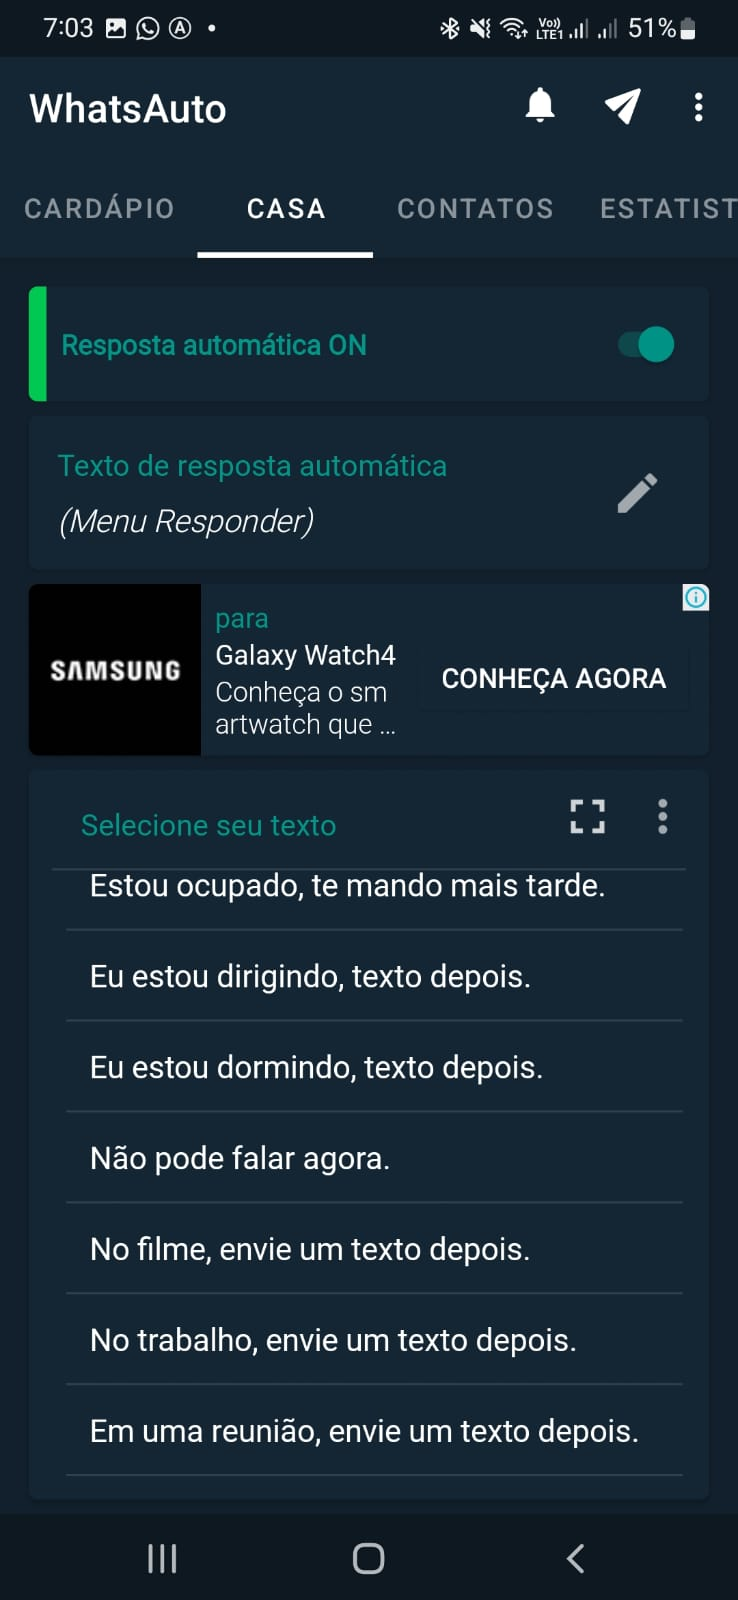
\includegraphics[width=6cm,height=8cm]{Partes/Imagens/Menu ligar 1.jpeg}
\caption{Fonte: Whatsauto (2022).}
\end{subfigure}%
\end{figure}

         E na parte do "texto de resposta automática", colocaremos a opção "Menu Responder", como mostra na imagem abaixo:

\begin{figure}[!htb]
\centering
\captionsetup[subfigure]{labelformat=empty}
\caption{``Menu Ligar 2''}
\begin{subfigure}{.5\textwidth}
\centering
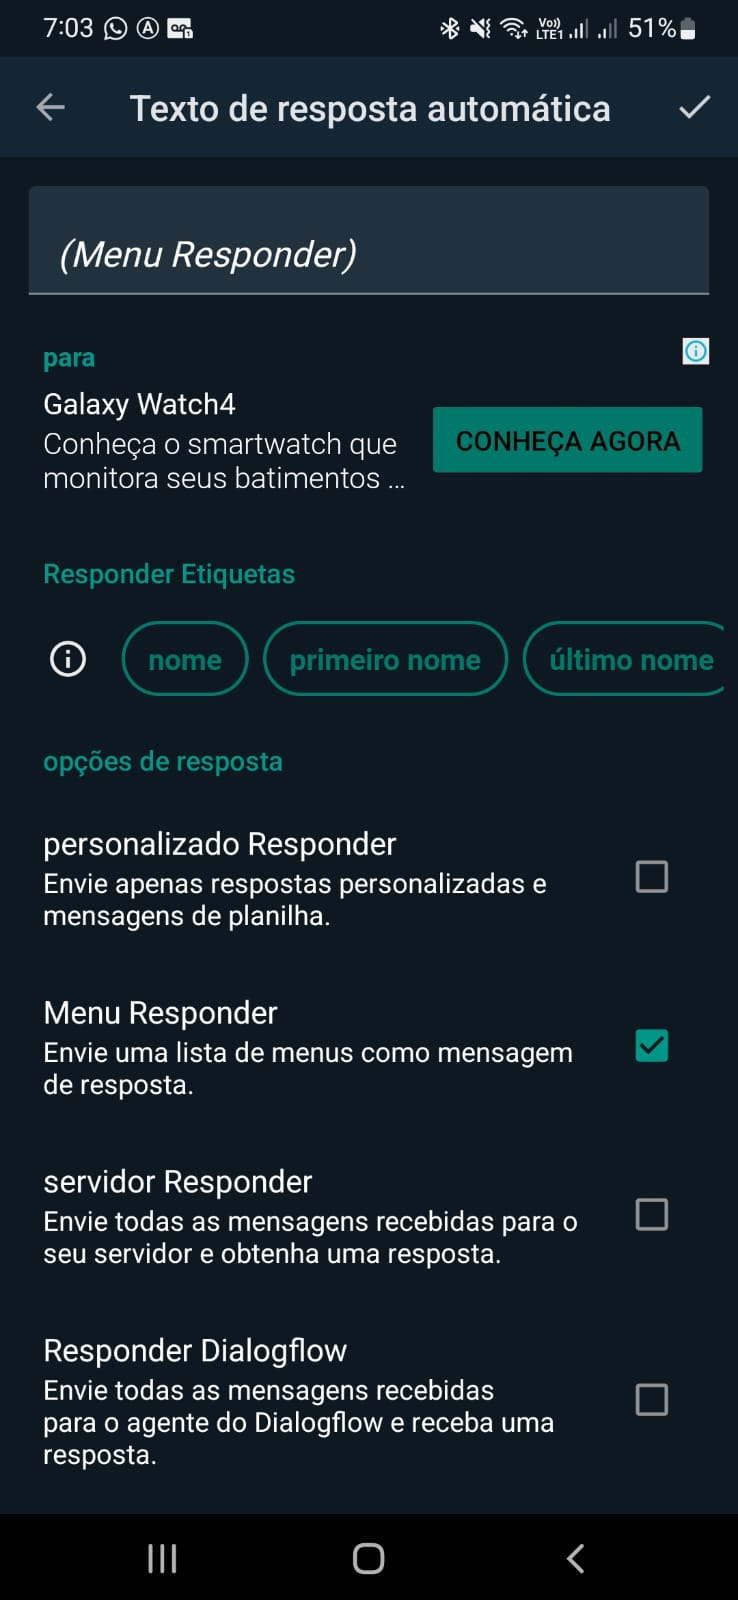
\includegraphics[width=6cm,height=8cm]{Partes/Imagens/Menu Ligar 2.jpeg}
\caption{Fonte: Whatsauto (2022).}
\end{subfigure}%
\end{figure}
\newpage
  
\section{Testes do Bot}
\subsection{Plano de testes:}

    Basicamente nós coletamos os feedbacks sobre a qualidade das informações passadas pelo BOT, entendimento de modo geral e usabilidade do layout do chat de WhatsApp.\\
	Diferente de outros BOTs, o nosso não possui a ferramenta de coleta de informações pessoais do usuário por meio de chat, nem uma IA \cite{ia}, para identificação linguística para maior aproximação com um atendente real, o que iria deixar mais natural e dinâmico as conversas com os usuários.\\
	Nós enviamos o link para algumas pessoas não envolvidas diretamente com nosso trabalho para testarmos todos os passos descritos acima. Obtivemos um resultado satisfatório e bem informativo, algumas criticas foram descritas, estamos fazendo de tudo para a correção futura.
\item \textbf{CRÍTICAS}: \\
Não tinha mensagem final ao parar de conversar com o BOT. \\
Falta do link na página do Instagram.\\
\item \textbf{ELOGIOS}: \\
“Um bom BOT bem útil, fácil de usar, tem só um atraso na resposta, mas nada que seja ruim ou que atrapalhe”\\
“No geral, está funcionando muito bem. Está bem resumido, porém explicativo”

\subsection{Resultado do plano de Testes:}

Foram feitos 8 testes com pessoas não relacionadas com nosso trabalho, 2 delas relataram problemas com o link do Instagram, o que nós não sabemos o porquê ocorreu. Várias ideias foram sugeridas pelos responsáveis pelos testes e algumas das ideias foram implementadas, por exemplo:\\
- Menu para sair da conversa\\
- Mensagem final agradecendo o teste e indicando nossa Pagina no Instagram. \\

\begin{figure}[!htb]
\centering
\captionsetup[subfigure]{labelformat=empty}
\caption{``Gráfico Pizza''}
\begin{subfigure}{.5\textwidth}
\centering
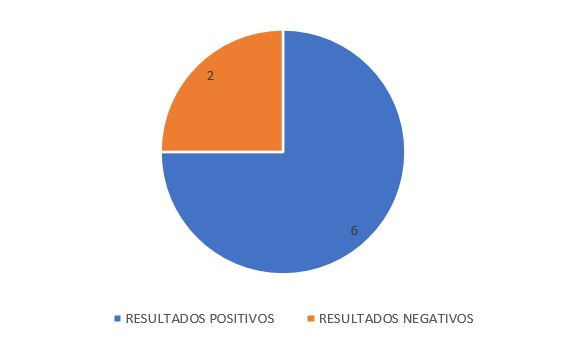
\includegraphics[width=8cm,height=6cm]{Partes/Imagens/Pizza.jpeg}
\caption{Fonte: Criado pelo autor (2022).}
\end{subfigure}%
\end{figure}

\newpage

\subsection{Imagens dos Testes:}

\begin{figure}[!htb]
\centering
\captionsetup[subfigure]{labelformat=empty}
\caption{``Teste 1''}
\begin{subfigure}{.5\textwidth}
\centering
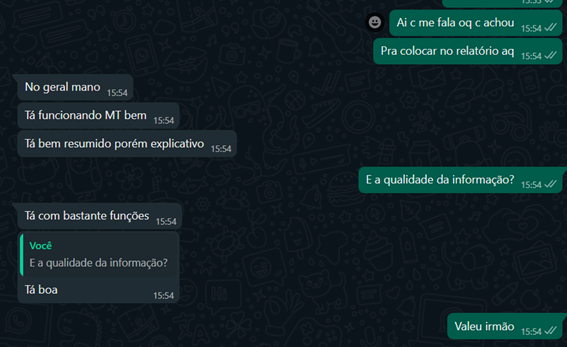
\includegraphics[width=6cm,height=8cm]{Partes/Imagens/teste 1.png}
\caption{Fonte: Criada pelo autor (2022).}
\end{subfigure}%
\end{figure}

\begin{figure}[!htb]
\centering
\captionsetup[subfigure]{labelformat=empty}
\caption{``Teste 2''}
\begin{subfigure}{.5\textwidth}
\centering
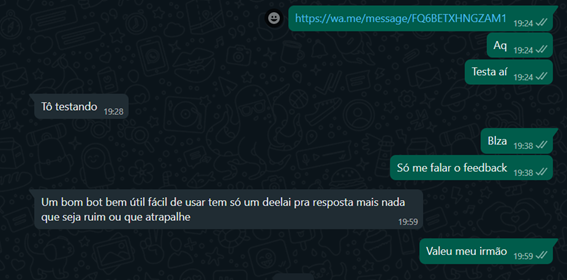
\includegraphics[width=6cm,height=8cm]{Partes/Imagens/teste 2.png}
\caption{Fonte: Criada pelo autor (2022).}
\end{subfigure}%
\end{figure}

\begin{figure}[!htb]
\centering
\captionsetup[subfigure]{labelformat=empty}
\caption{``Teste 3''}
\begin{subfigure}{.5\textwidth}
\centering
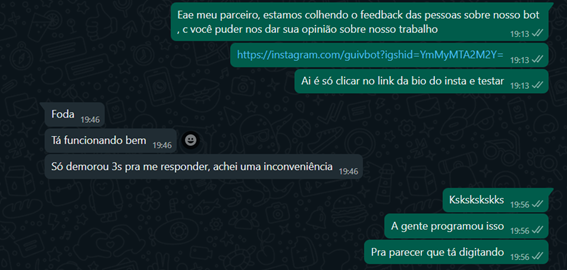
\includegraphics[width=6cm,height=8cm]{Partes/Imagens/teste 3.png}
\caption{Fonte: Criada pelo autor (2022).}
\end{subfigure}%
\end{figure}

\newpage

\subsection{Conclusões dos Testes:}

No geral foram obtidos bons resultados em todos os aspectos, as críticas foram recebidas muito bem. O resultado foi satisfatório. 

\section{Disponibilização do BOT}

 A plataforma que foi escolhida no projeto tem uma ampla vasta de disponibilização, porém a escolhida foi o WhatsApp, pois é um local onde os usuários tem mais acesso e disponibilidade para usar.
		
\end{itemize}

